% 2009 年湖南卷理科第 18 题：正三棱柱 ABC-A1B1C1，D 为 A1B1 中点，E 在 A1C1 上且 DE⊥AE。
% 来源 PDF：普通高考/2009/2009湖南理.pdf，SHA-256 0237bd2509e6645937e3473eabb63dba69098024fb6f451cb44ef8ac0e3165c1。
% 原页：第 1 页（A3 三栏）第 3 栏中部，书页码 527。
% 重绘依据：按原页斜视方向重绘；正三棱柱底面边长 AB=4、侧棱 AA1=2√2（图上按示意比例）。
%   可见：A1A、AB、BB1、A1B1、A1C1、C1B1 为实线；被遮挡的 AC、CC1、CB 为虚线。
%   辅助线 A1D、A1E、AD、AE、DE 按原页画虚线；D 在 A1B1 上，E 在 A1C1 上（AE:EC≈1:3）。
%   投影取 (x,y,z) -> (x+0.13y, z+0.45y)。
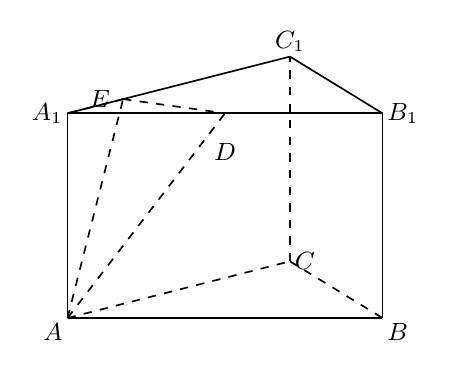
\begin{tikzpicture}[semithick, every node/.style={inner sep=1.5pt, font=\small}]
  \coordinate (A)  at (0.000,0.000);
  \coordinate (B)  at (4.000,0.000);
  \coordinate (C)  at (2.825,0.720);
  \coordinate (A1) at (0.000,2.600);
  \coordinate (B1) at (4.000,2.600);
  \coordinate (C1) at (2.825,3.320);
  \coordinate (D)  at (2.000,2.600);
  \coordinate (E)  at (0.706,2.780);

  % 可见棱
  \draw (A1) -- (A);
  \draw (A) -- (B);
  \draw (B) -- (B1);
  \draw (A1) -- (B1);
  \draw (A1) -- (C1);
  \draw (C1) -- (B1);

  % 被遮挡的棱
  \draw[dashed] (A) -- (C);
  \draw[dashed] (C) -- (C1);
  \draw[dashed] (C) -- (B);

  % 辅助线
  \draw[dashed] (A1) -- (D);
  \draw[dashed] (A1) -- (E);
  \draw[dashed] (A) -- (D);
  \draw[dashed] (A) -- (E);
  \draw[dashed] (E) -- (D);

  % 标注
  \node[left] at (A1) {$A_1$};
  \node[right] at (B1) {$B_1$};
  \node[above] at (C1) {$C_1$};
  \node[below left] at (A) {$A$};
  \node[below right] at (B) {$B$};
  \node[right] at (C) {$C$};
  \node[below=9pt] at (D) {$D$};
  \node[left=3pt] at (E) {$E$};
\end{tikzpicture}
